\documentclass{beamer}
\usetheme{Madrid}
\usepackage[T2A]{fontenc}
\usepackage[utf8]{inputenc}
\usepackage[english,russian]{babel}
\usepackage{graphicx}
\usepackage{xcolor}
\usepackage{amsmath}
\usepackage{mathtools}
\usepackage{bm}
\usepackage{bbm}
\usepackage{pifont}
\usepackage{physics}
\usepackage{hyperref}
\usepackage{appendixnumberbeamer}
\usepackage[backend=biber]{biblatex}
\addbibresource{rudakov-etapipi-2025.bib}

\title[$e^+e^-\rightarrow{}\eta\pi^+\pi^-$]{Изучение процесса $e^+e^-\to\eta\pi^+\pi^-$ с детектором КМД-3}
\author{Грибанов Сергей Сергеевич}
\date{\today}


\begin{document}

\frame{\titlepage}

\begin{frame}
  \frametitle{Коллайдер ВЭПП-2000}
\end{frame}

\begin{frame}
  \frametitle{Детектор КМД-3}
\end{frame}

\begin{frame}
  \frametitle{Мотивация}
\end{frame}

\begin{frame}
  \frametitle{Процесс $e^+e^-\to\eta\pi^+\pi^-$}
  \scriptsize
  \centering
  \textbf{Промежуточные состояния:}

  \begin{minipage}[t]{0.4\linewidth}
    \textit{Достоверно наблюдаются:}
    \begin{itemize}
    \item $\rho(770)\eta$
    \item $a_2(1320)\pi$
    \end{itemize}
  \end{minipage}
  \begin{minipage}[t]{0.4\linewidth}
    \textit{Изучались, но дают малый вклад:}
    \begin{itemize}
      \item $\omega(770)\pi$~($\rho$-$\omega$ смешивание)
      \item $\rho(1450)\pi$
      \item $\rho(1700)\pi$
    \end{itemize}
  \end{minipage}
\end{frame}

\begin{frame}
  \frametitle{Критерии отбора событий}
  \scriptsize
  \begin{itemize}
    \item Наличие двух центральных треков
    \item Наличие двух или более фотонов с энергиями больше $50\text{ МэВ}$.
    \item Суммарное энерговыделение кандидатов на $\pi^+$ и $\pi^-$ в калориметре меньше
      $0.4 + 0.25\times(\sqrt{s} - 1.2)$~ГэВ для подавления событий $e^+e^-$ рассеяния.
    % \item В зависимостях $\dv{E(p)}{x}$ для кандидатов в $\pi^{\pm}$ вырезается (мягко) области
    %   отвечающие $\pi$-мезонам.
    \item Кинематическая реконструкция\footfullcite{Gribanov_2023}
      в гипотезе $e^+e^-\rightarrow\pi^+\pi^-\gamma\gamma$: фит должен сойтись
      и $\chi^2<40$.
    \item Кинематическая реконструкция в гипотезе $e^+e^-\rightarrow\pi^+\pi^-\gamma\gamma\gamma\gamma_{\text{lost}}$. Одна
      пара фотонов складывается в $\pi^0$ (для которой $\chi^2$ меньше). Требуется, чтобы
      либо фит не сошелся, либо фит сошелся и $\chi^2>20$.
    \item Кинематическая реконструкция в гипотезе $e^+e^-\rightarrow\eta\pi^+\pi^-$, $\eta\rightarrow\gamma\gamma$. Требуется,
      чтобы фит сошелся, но никаких ограничений на $\chi^2$ не накладывается. Нужна
      для того, чтобы в амплитудном фите четырех-импульс двух фотонов
      соответствовал четырех-импульсу $\eta$-мезона.
    \item Для амплитудного анализа также накладывается ограничение на инвариантную
      массу двух фотонов после фита в первой гипотезе : $0.51\text{ ГэВ}/c^2 < m_{\gamma\gamma} < 0.59\text{ ГэВ}/c^2$.
  \end{itemize}
\end{frame}

\begin{frame}
  \frametitle{Амплитудный анализ}
\end{frame}

\begin{frame}
  \frametitle{Учет фона}
\end{frame}

\begin{frame}
  \frametitle{Сравнение спектров, $\sqrt{s}\approx{1.9}\text{ ГэВ}$}
  \begin{minipage}[t]{0.48\linewidth}
    \begin{figure}
      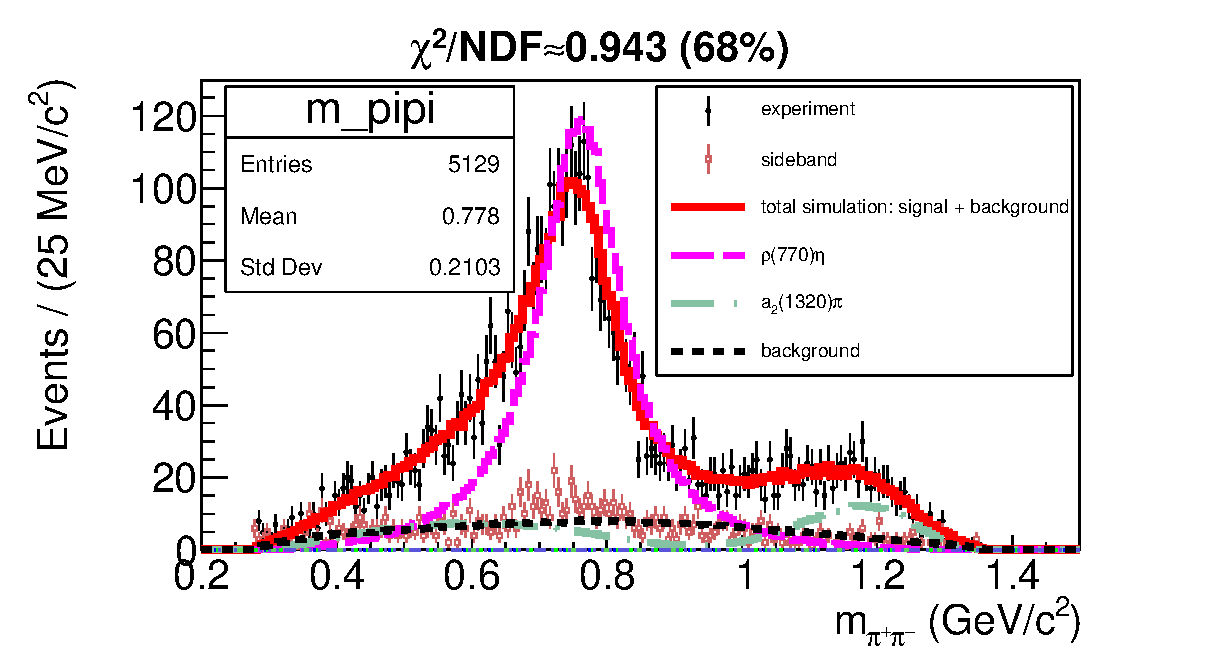
\includegraphics[width=\linewidth]{figures/m_pipi_g950.eps}
    \end{figure}
  \end{minipage}
  \begin{minipage}[t]{0.48\linewidth}
    \begin{figure}
      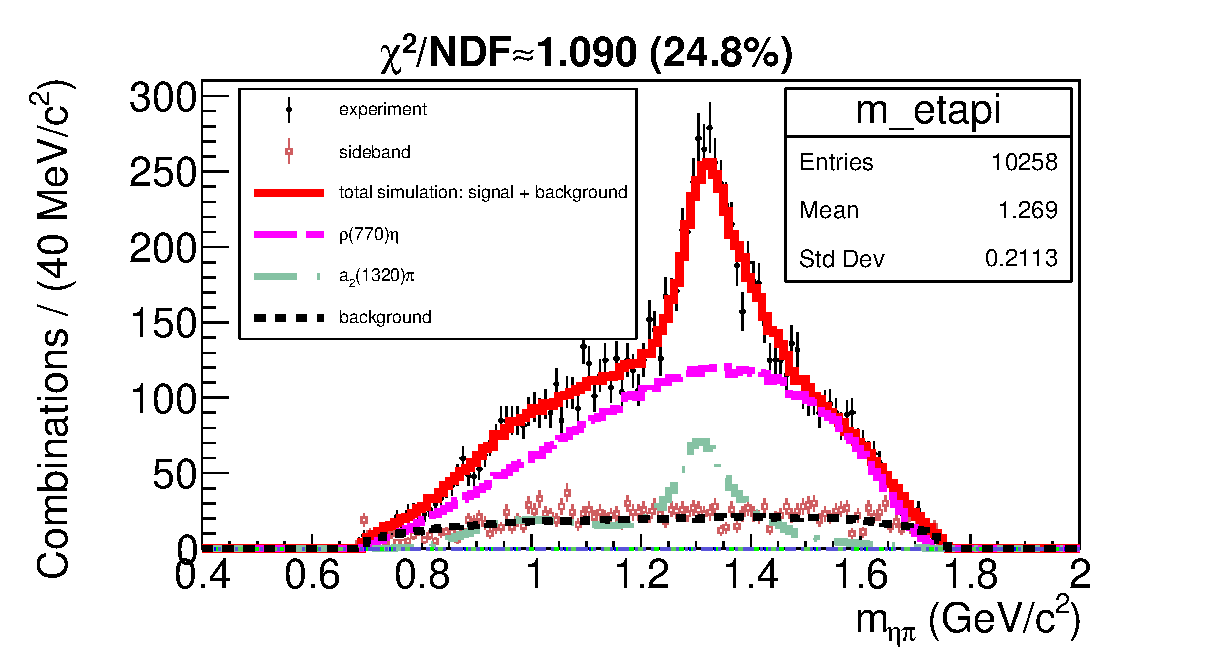
\includegraphics[width=\linewidth]{figures/m_etapi_g950.eps}
    \end{figure}
  \end{minipage}
  \begin{minipage}[t]{0.48\linewidth}
    \begin{figure}
      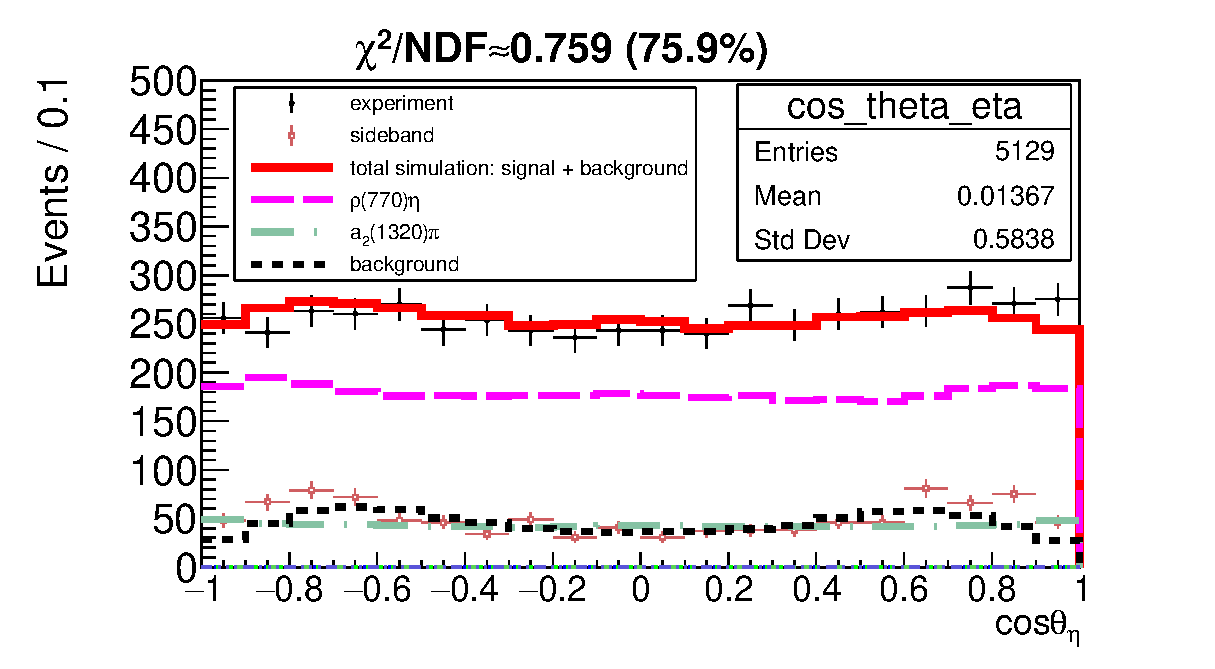
\includegraphics[width=\linewidth]{figures/cos_theta_eta_g950.eps}
    \end{figure}
  \end{minipage}
  \begin{minipage}[t]{0.48\linewidth}
    \begin{figure}
      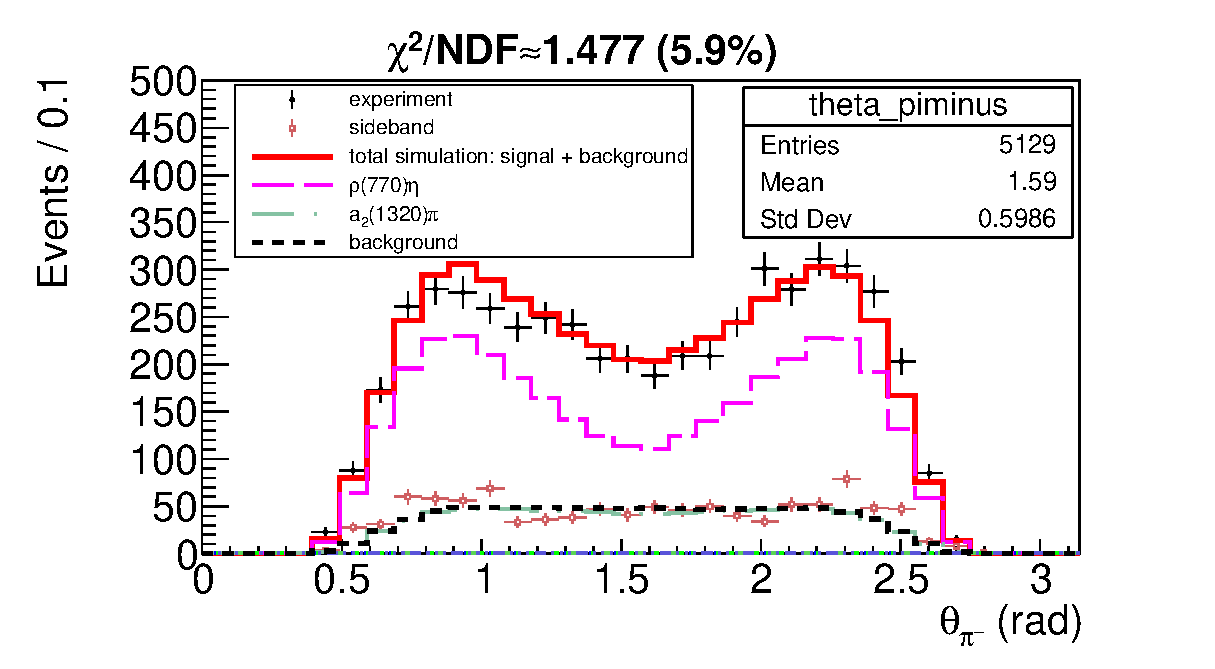
\includegraphics[width=\linewidth]{figures/theta_piminus_g950.eps}
    \end{figure}
  \end{minipage}
\end{frame}

\begin{frame}
  \frametitle{Сравнение спектров, $\sqrt{s}\approx{1.4}\text{ ГэВ}$}
  \begin{minipage}[t]{0.48\linewidth}
    \begin{figure}
      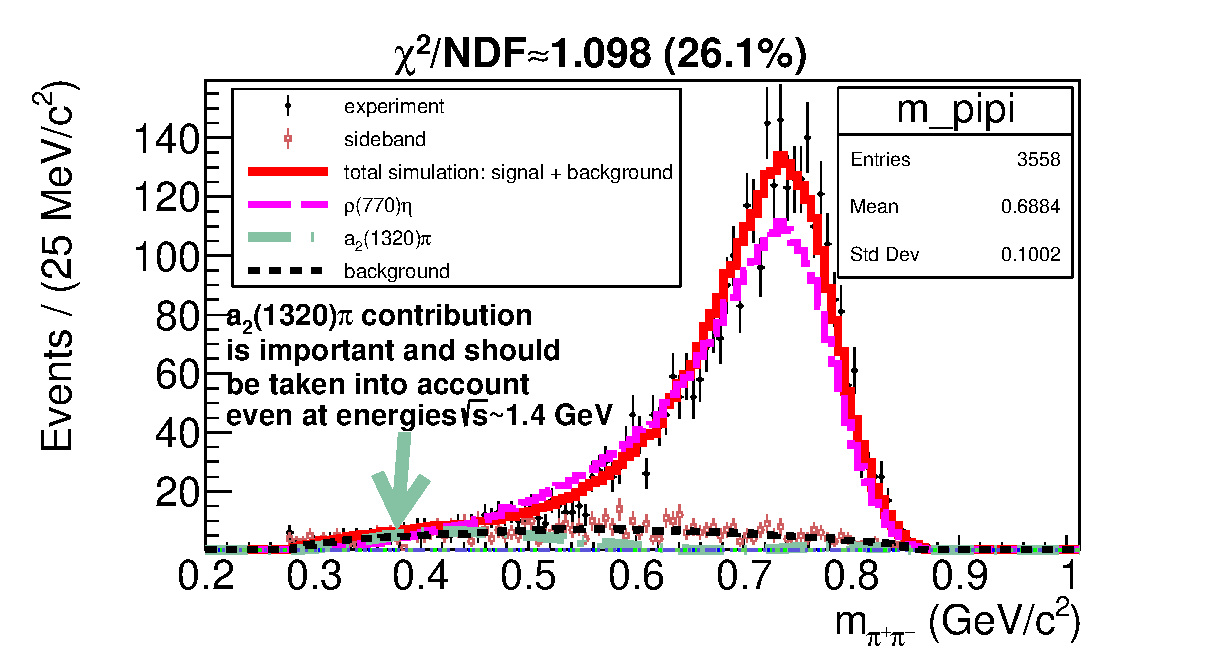
\includegraphics[width=\linewidth]{figures/m_pipi_g705.eps}
    \end{figure}
  \end{minipage}
  \begin{minipage}[t]{0.48\linewidth}
    \begin{figure}
      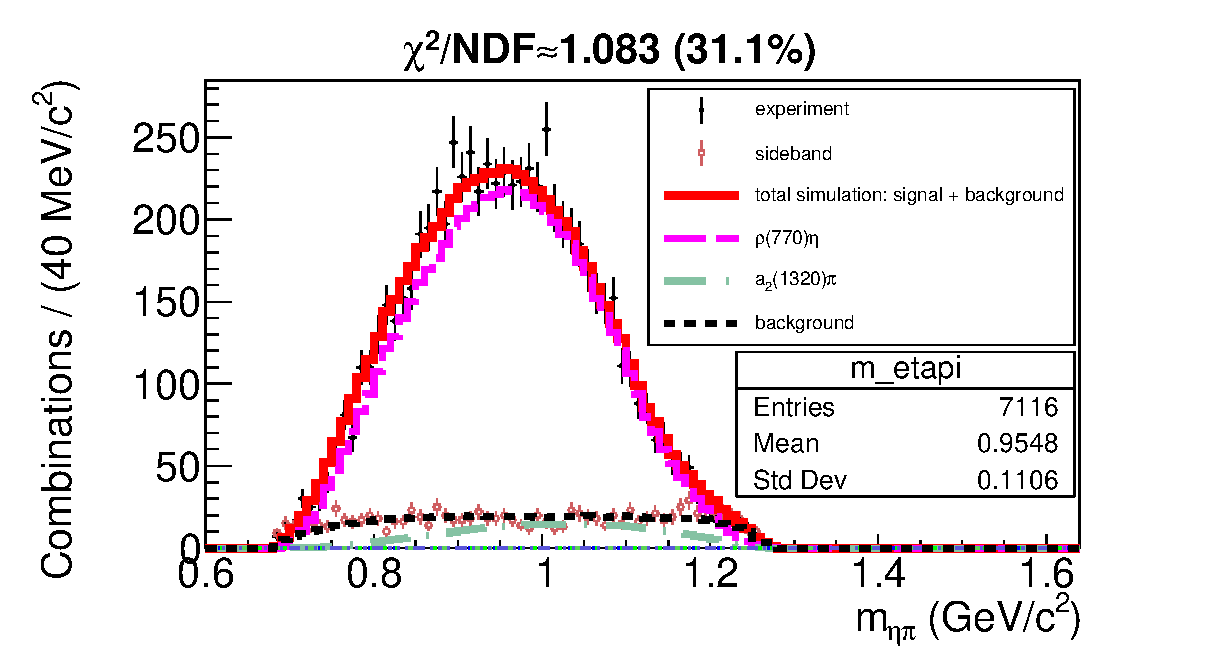
\includegraphics[width=\linewidth]{figures/m_etapi_g705.eps}
    \end{figure}
  \end{minipage}
  \begin{minipage}[t]{0.48\linewidth}
    \begin{figure}
      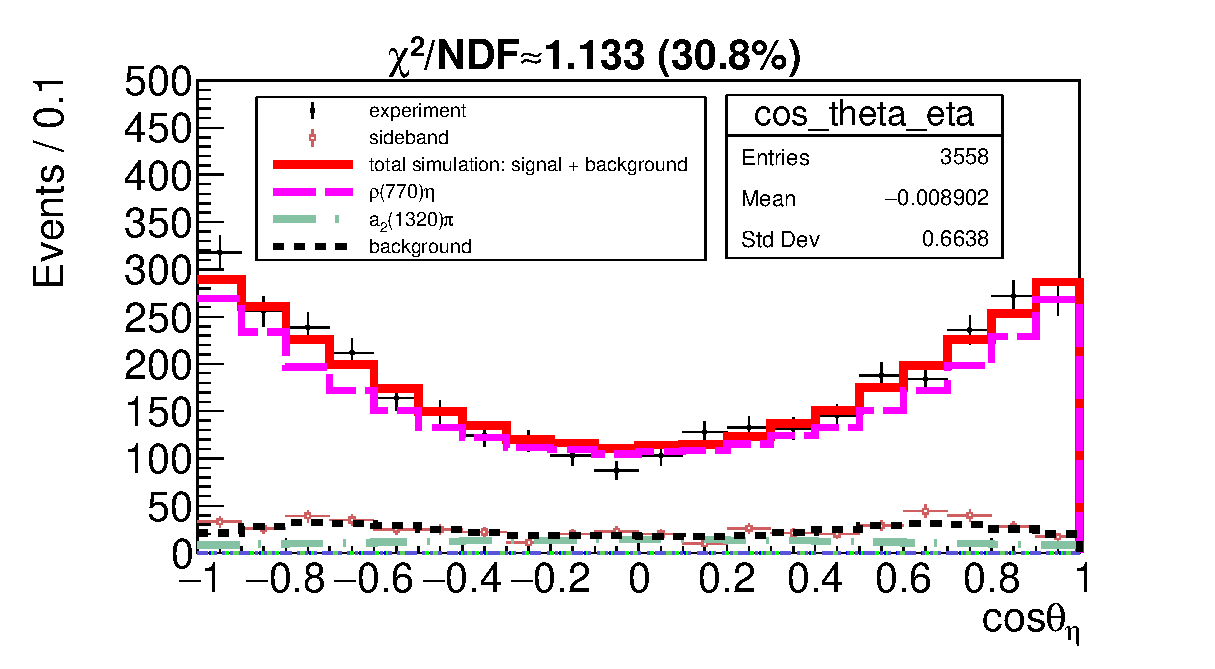
\includegraphics[width=\linewidth]{figures/cos_theta_eta_g705.eps}
    \end{figure}
  \end{minipage}
  \begin{minipage}[t]{0.48\linewidth}
    \begin{figure}
      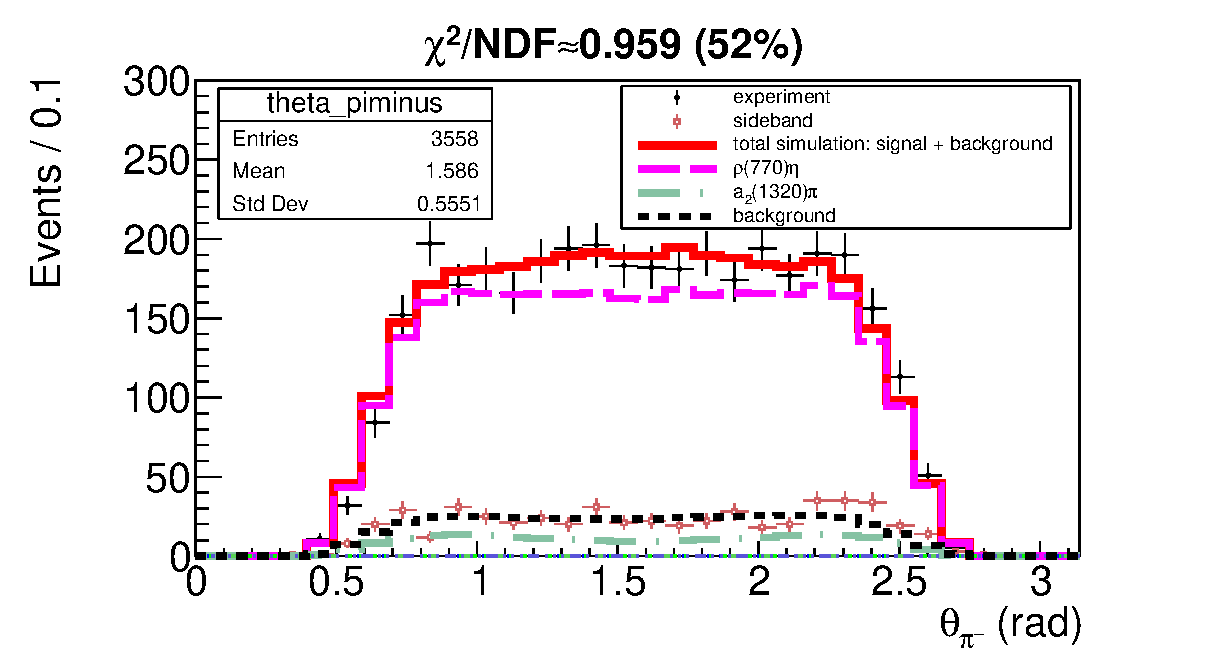
\includegraphics[width=\linewidth]{figures/theta_piminus_g705.eps}
    \end{figure}
  \end{minipage}
\end{frame}


\begin{frame}
  \frametitle{Сечение}
  \begin{minipage}[t]{0.48\linewidth}
    \begin{figure}
      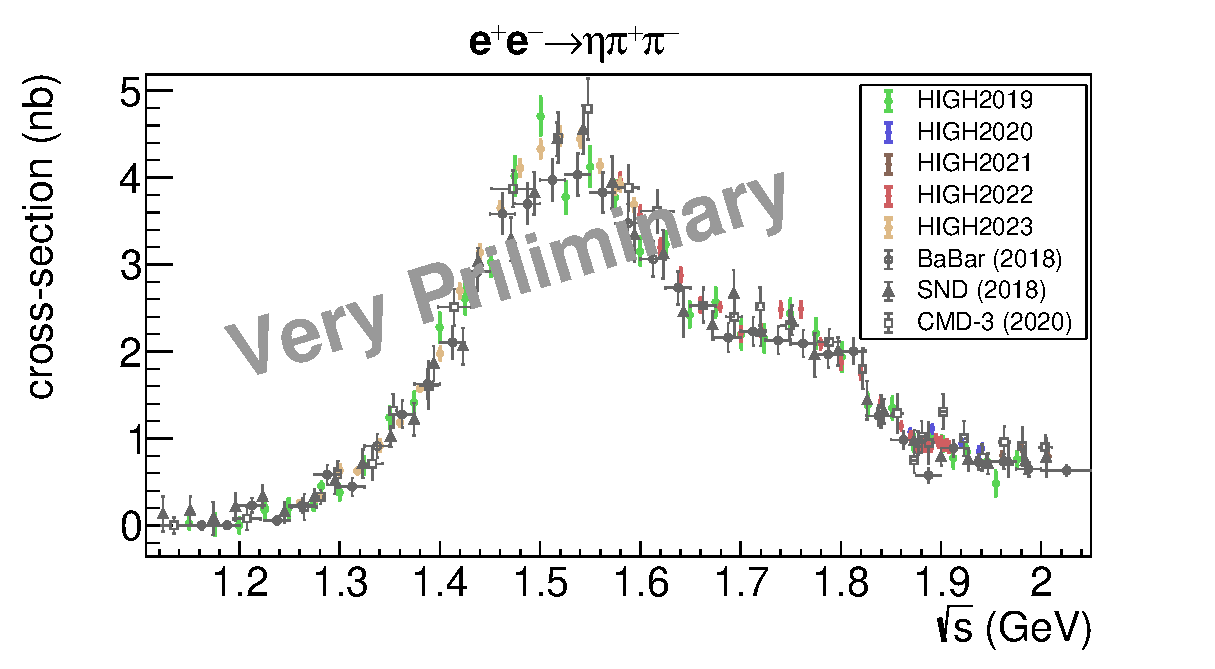
\includegraphics[width=\linewidth]{figures/bcs_etapipi.eps}
    \end{figure}
  \end{minipage}
  \begin{minipage}[t]{0.48\linewidth}
    \begin{figure}
      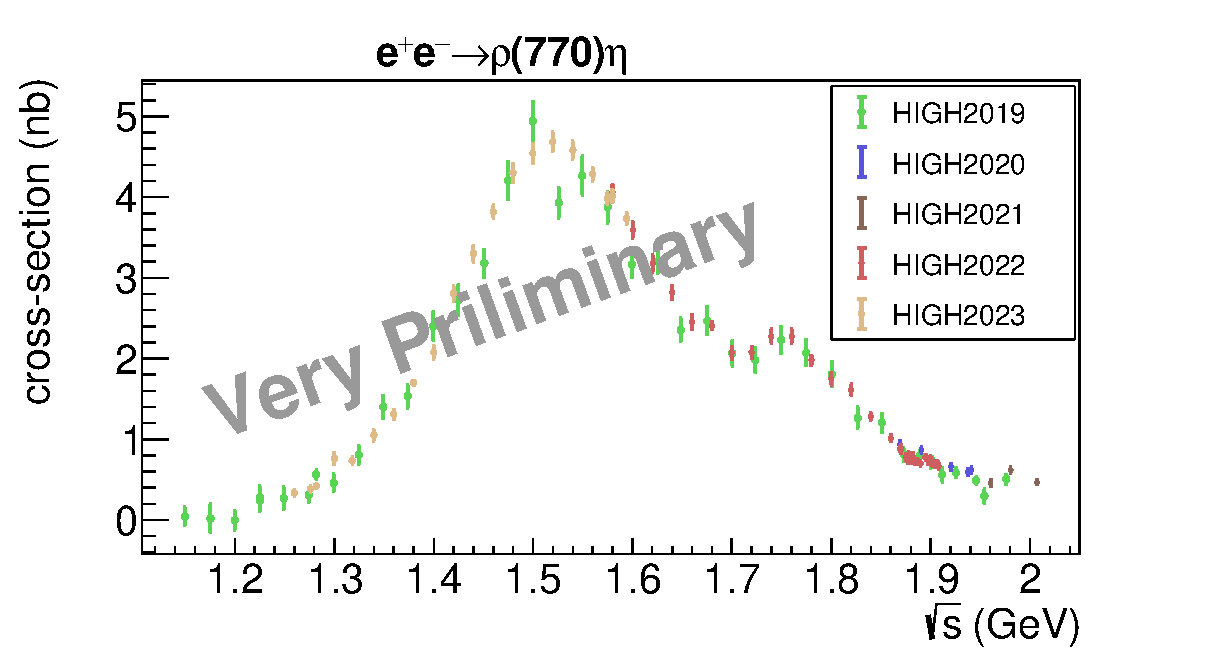
\includegraphics[width=\linewidth]{figures/bcs_partial_rhoeta.eps}
    \end{figure}
  \end{minipage}
  \begin{minipage}[t]{0.48\linewidth}
    \begin{figure}
      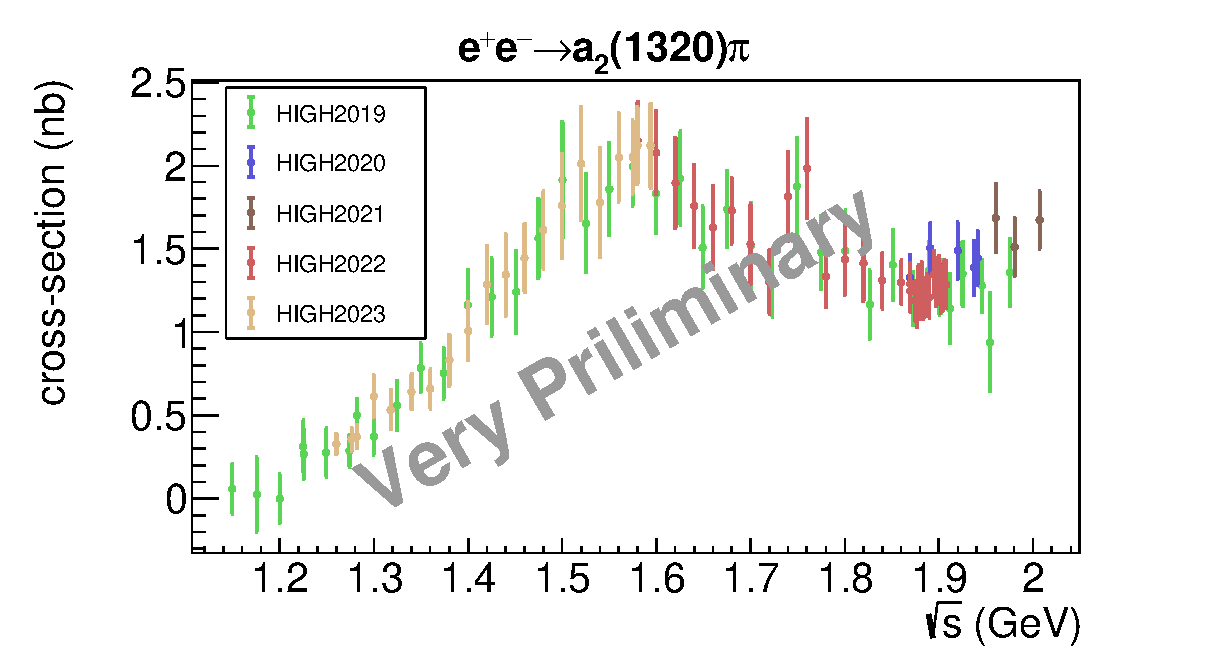
\includegraphics[width=\linewidth]{figures/bcs_partial_a2pi.eps}
    \end{figure}
  \end{minipage}
\end{frame}

\begin{frame}
  \frametitle{Уточнение модели фона}
\end{frame}


\end{document}
